\documentclass{article}
\usepackage{apamposter_1}
\usepackage[square,numbers]{natbib}
\usepackage{lmodern}
\usepackage{textpos}
\setcounter{secnumdepth}{2}
\newcommand{\nb}[1] {\textcolor{red}{#1}}
\setlength{\TPHorizModule}{1in}
\setlength{\TPVertModule}{1in}
\begin{document}
\bibliographystyle{plainnat}
%\begin{center}
%
% Start of title...
%
% switch into sans-serif for title

\begin{textblock}{62}(0,0)

%\textblockcolor{white}

\begin{center}

\vspace{5mm}\def\myfig#1{\begin{center}\includegraphics[width=\graphicswidth]{#1}\end{center}}

{\VeryHuge\color{black} \textbf{Investigation of MHD Mode Structure in Shaped HBT-EP Discharges}}

\vspace{15mm}
\rm
\sf
\LARGE\textbf{\color{lnavy}
P. Byrne$^\dagger$, J. P. Levesque, M. E. Mauel, Q. Peng, D. J. Rhodes, P. E. Hughes, G. A. Navratil  \hspace{2in} \emph{Columbia University}}\\

\vspace{5mm}

\end{center}
\end{textblock}
\begin{textblock}{12}(49,3)
\begin{flushright}

{\color{black}$^{\dagger}$email: {pjb2132@columbia.edu} }\hspace{.25in}

\end{flushright}
\end{textblock}

\begin{textblock}{3}(.2,.75)


\includegraphics[scale =.75]{CU_logo_exported.png}

\end{textblock}


\begin{textblock}{1}(57,.45)


\includegraphics[scale =1]{hbt_logo.png}

\end{textblock}


\vspace{100mm}
\hrule{}
\vspace{10mm}

% End of title, start of content..

\begin{multicols}{5}
\section{Abstract}
%\begin{itemize}
%\footnote{Levesque, \textit{et al.}, \textit{Nucl Fusion} \textbf{53}, 073037 (2013).}  \footnote{Maurer, et al., \textit{Plasma Phys Contr F} \textbf{53}, 074016 (2011).} 
We report on investigations into the effect on the structure of MHD kink modes of a newly installed poloidal field (PF) coil.  The coil allows the circular, limited HBT-EP to investigate plasmas that are shaped and diverted.  The coil shapes the high field side of the plasma up to and including imposing a PF null, without interfering with existing diagnostics and control systems. Shaping changes both the resonant helical characteristics of MHD instabilities\cite{Maurer} and the plasma response to external excitation and active control. In circular HBT-EP plasmas, multimode dynamics have been observed in naturally-rotating kink modes and during the response to 3D resonant magnetic perturbations\cite{Levesque, Shiraki}.  Work is ongoing to determine how the multimode dynamics of shaped plasmas differ from circular ones.\\
\section{Hardware and Capabilities}
\subsection{Magnetic Diagnostics and Control}
\begin{itemize}
\item HBT-EP has a passively stabilizing wall constructed of 20 independently positionable shells
\item Each shell is instrumented with two independently controlled saddle coils, allowing feedback on modes for excitation or control
\item 216 magnetic sensors form 2 poloidal arrays and 5 toroidal arrays
\subitem - 82 $B_r$ sensors, 134 $B_p$ sensors
\begin{center}
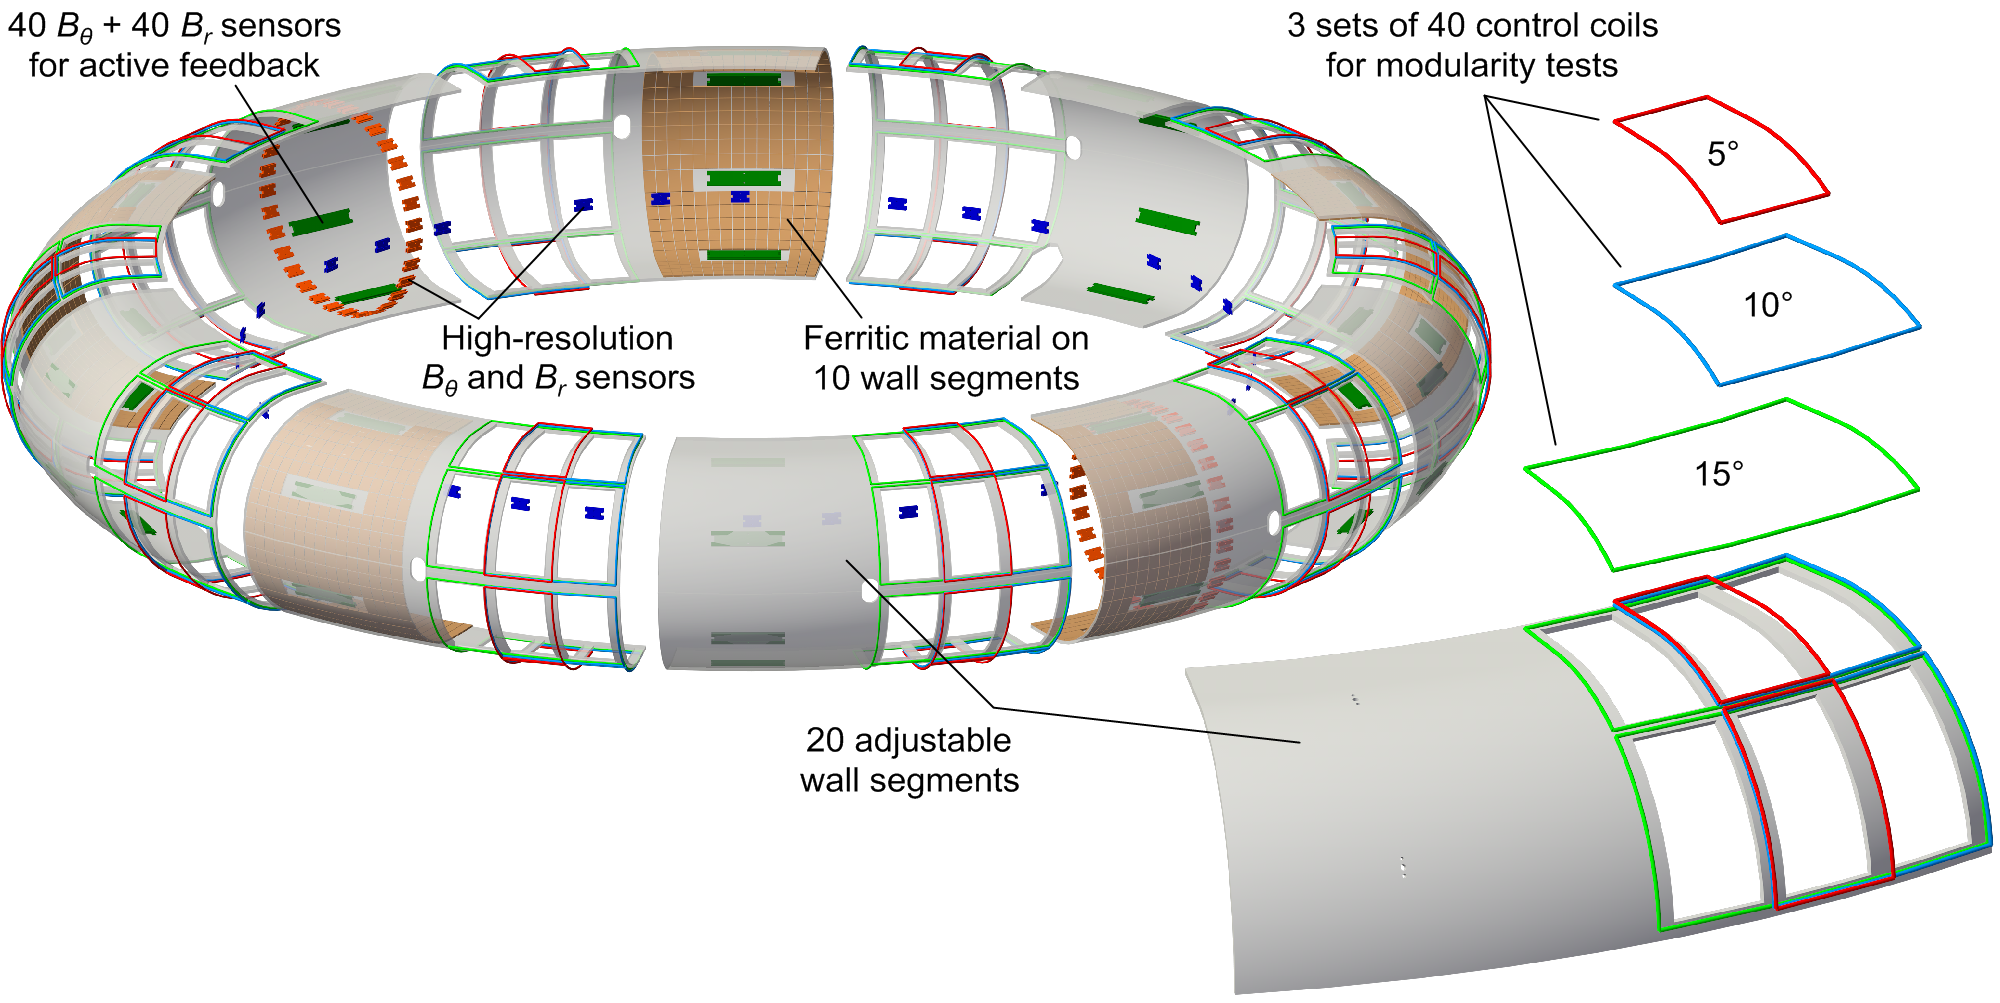
\includegraphics[width=0.9\columnwidth]{Plasma_with_sensors_FWall_concept_WithCCview}
\subsection{The Shaping Coil}
\end{center}
\item Diverts the plasma via a single null $30^{\circ}$ above the inboard midplane
\item 4 central coils carry co-Ip current, 2 sets of two flanking bundles carry contra-Ip current
\subitem - Reduced coupling to vacuum field coils and plasma diagnostics
\subitem - Shaping is locally imposed

\begin{center}
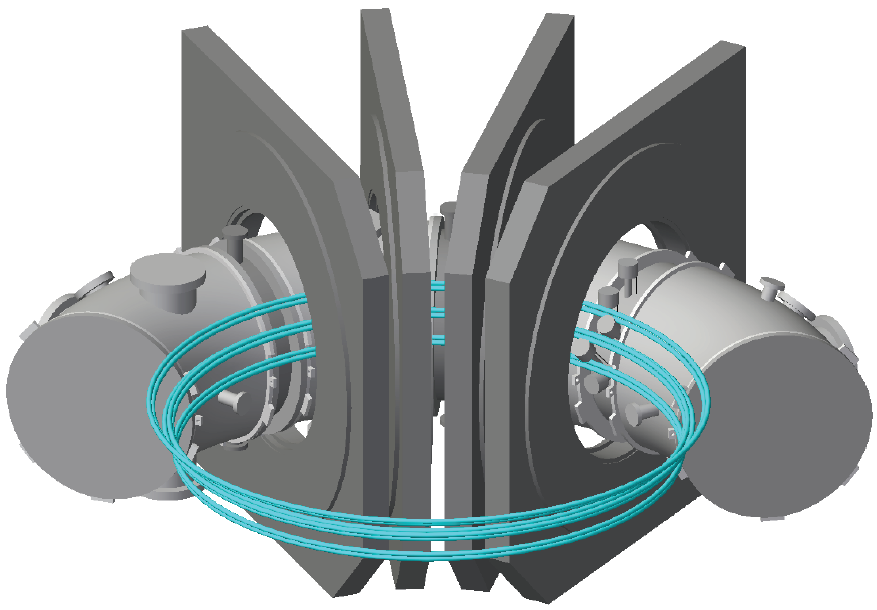
\includegraphics[width=0.9\columnwidth]{HBT_section_cropped}\\
\end{center}

\item Diversion has been measured directly via poloidal field inversions and confirmed by equilibrium reconstructions
\begin{center}
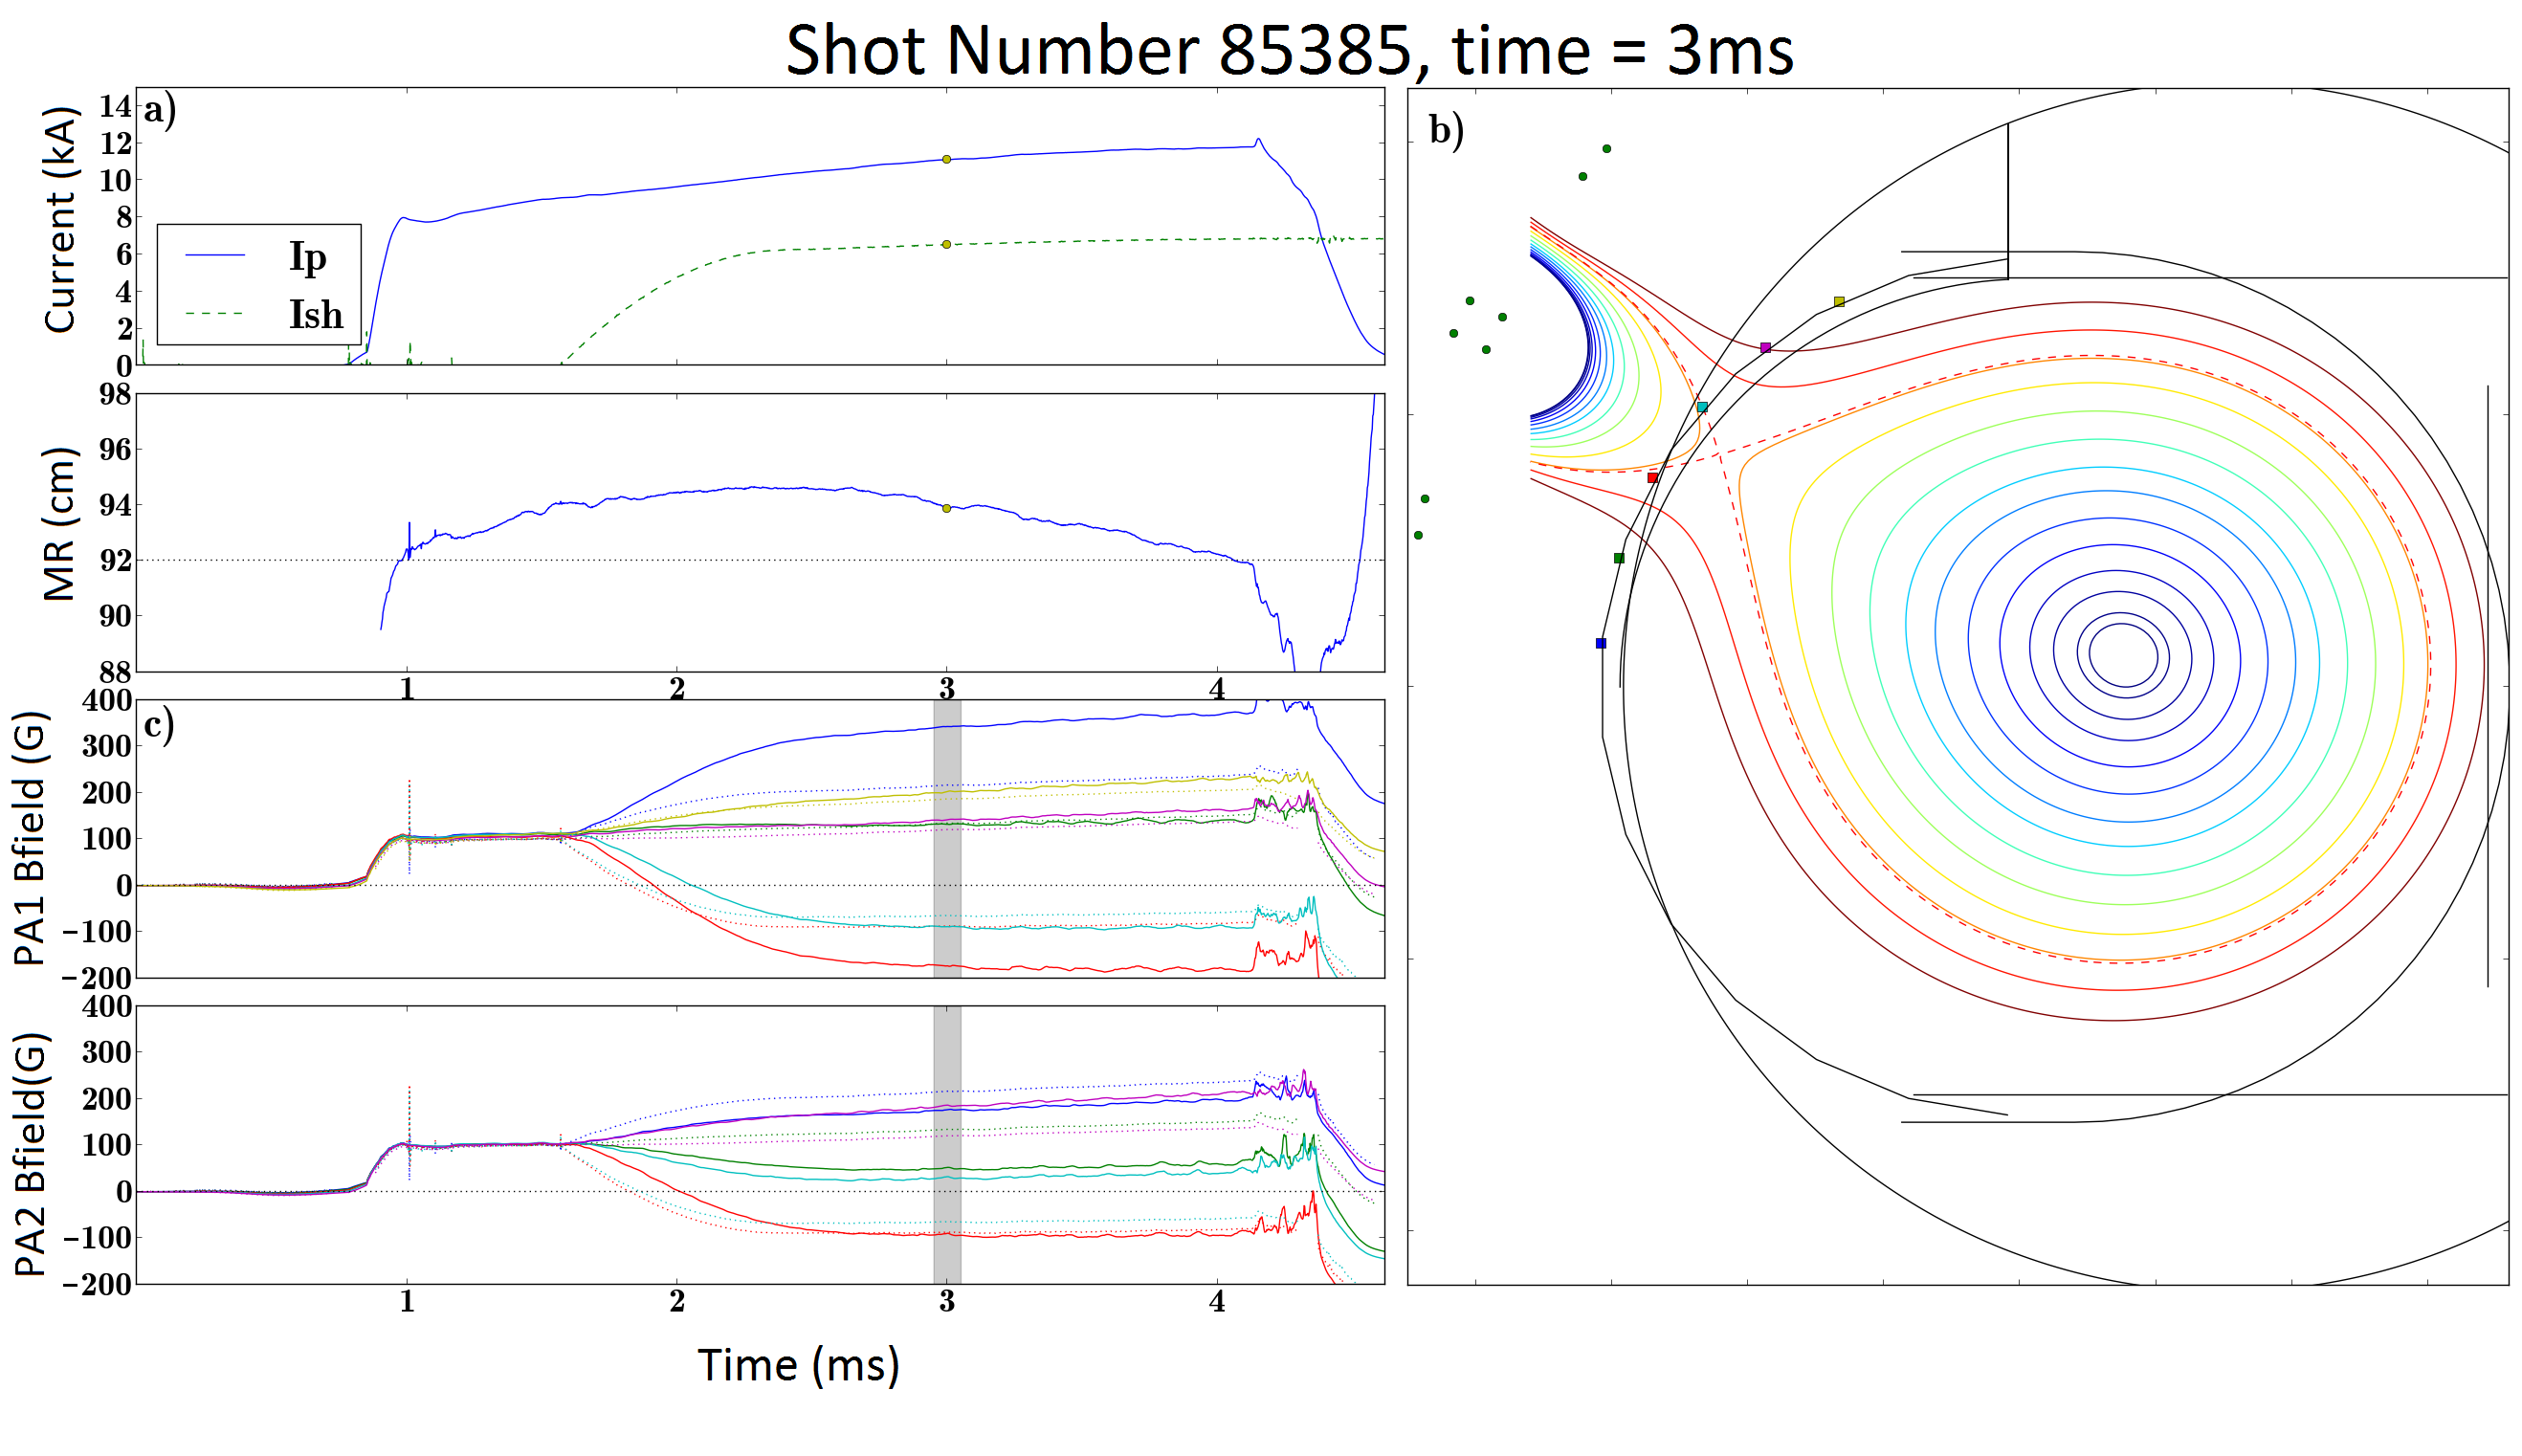
\includegraphics[width=1.05\columnwidth]{flux_surfaces_during_shaping85385_1}\\
\end{center}
\item Reversing the direction of shaping current is also possible, allowing investigation of 'bean-shaped' plasmas

\begin{center}
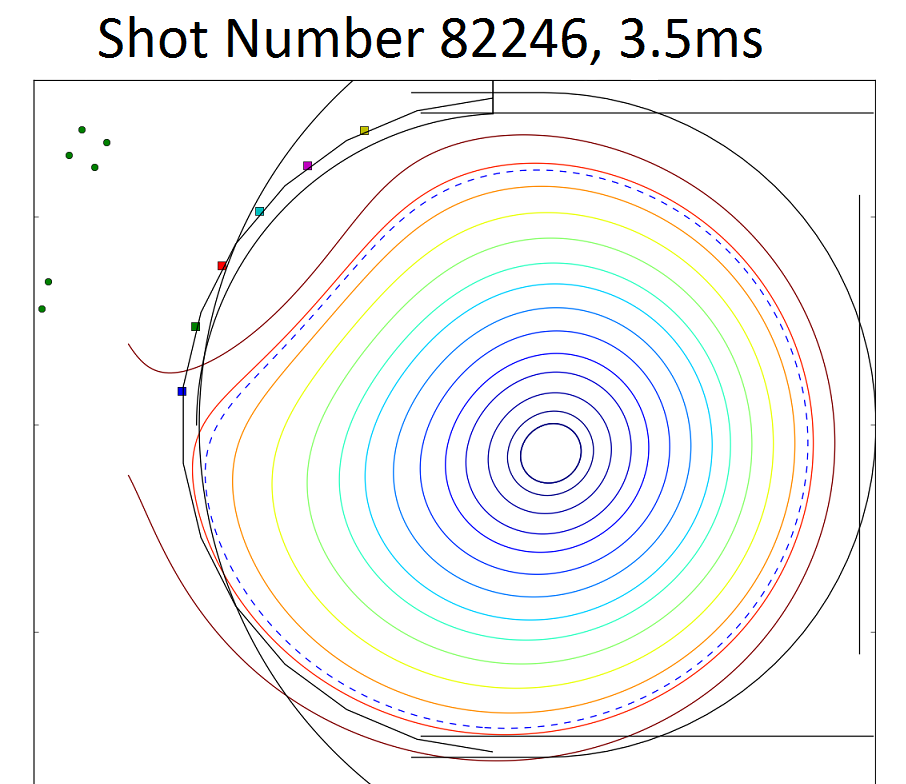
\includegraphics[width=0.6\columnwidth]{flux_surfaces_during_shaping_reverse_polarity}\\
\end{center}

\section{Mode Detection and Analysis}
\subsection{Sensor Data}

\item Magnetic fluctuations are observed with high poloidal and toroidal resolution
\begin{center}
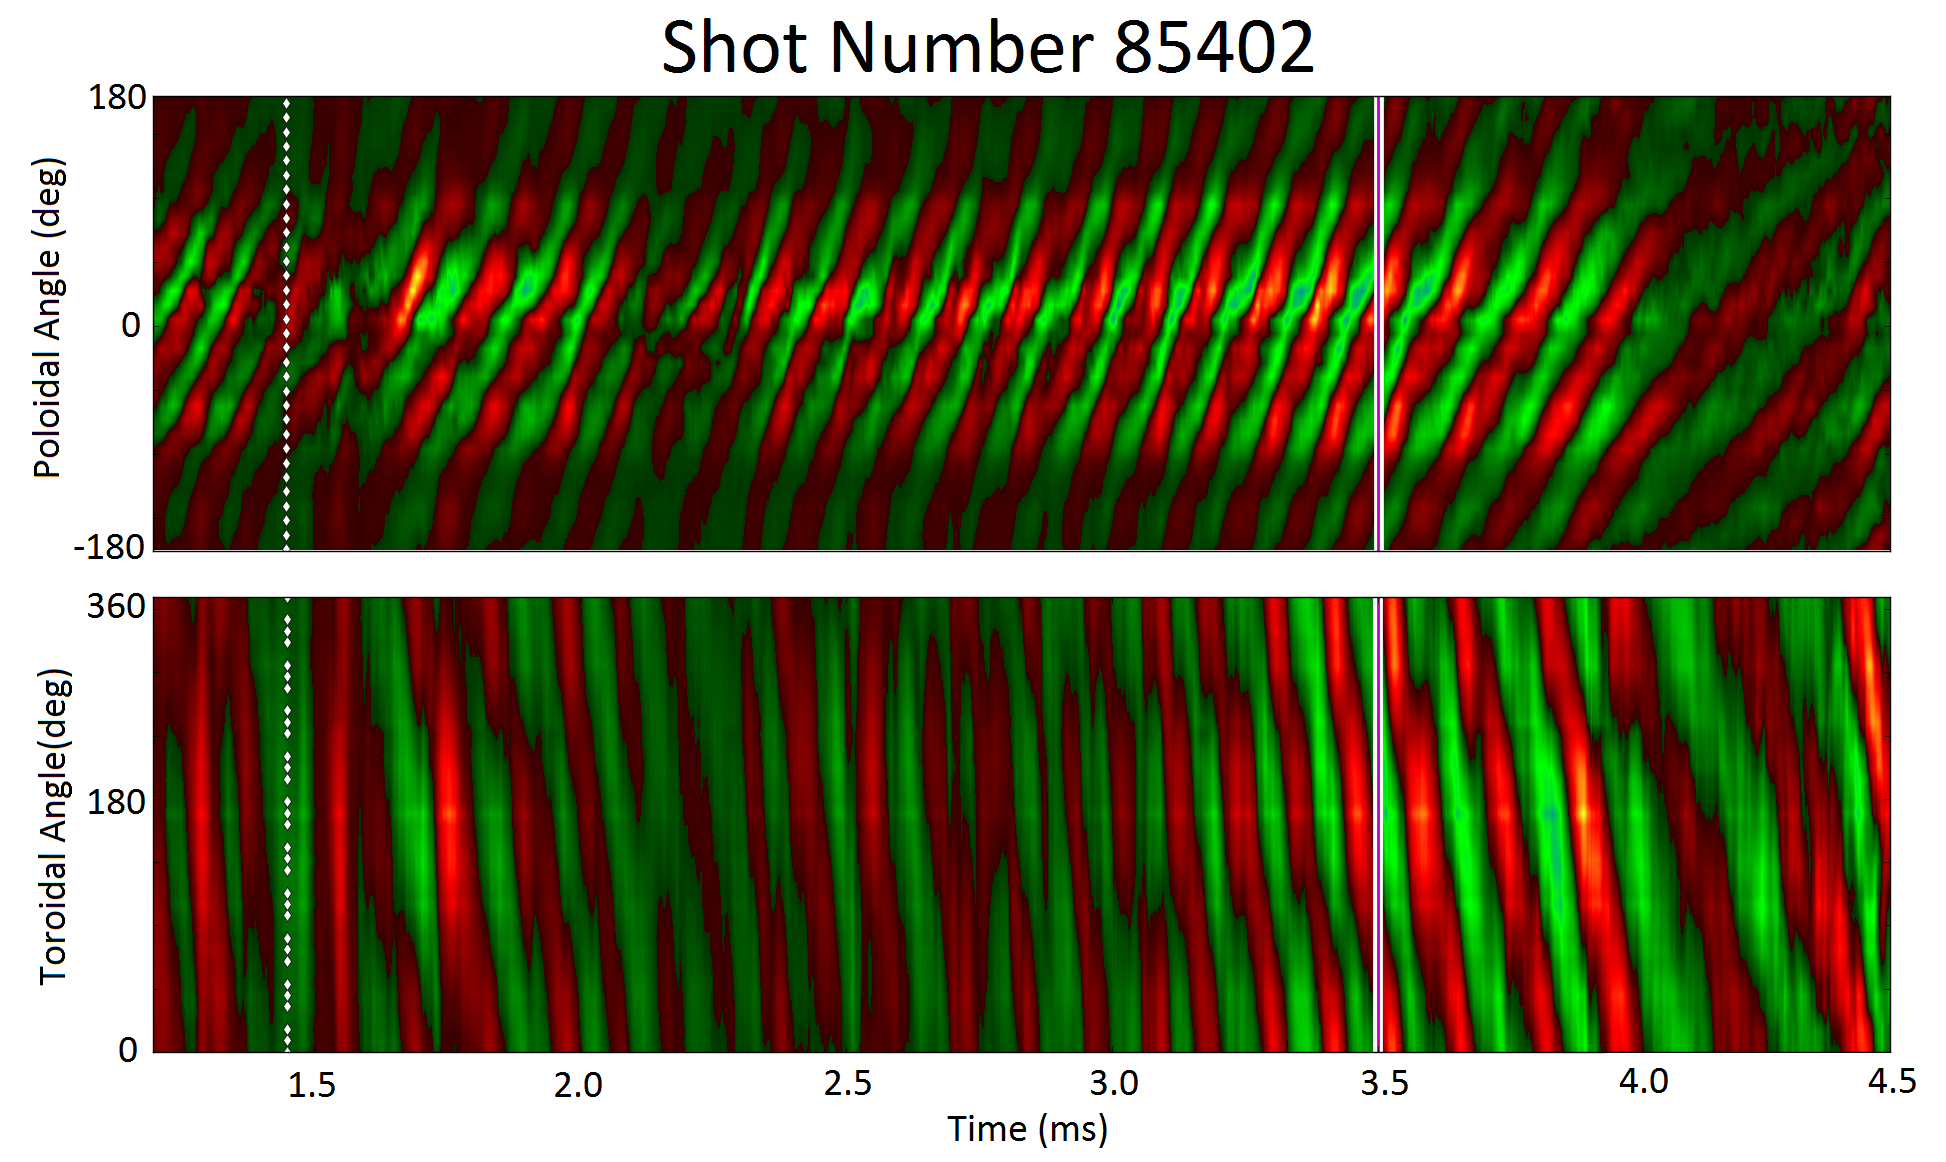
\includegraphics[width=1\columnwidth]
{stripeys_pol_and_tor_85402}\\
\end{center}
\item Fluctuations are often dominated by a single mode, visible by inspection
\subitem - Lower power modes are observed through Biorthogonal Decomposition\\
\subsection{Biorthogonal Decomposition}
\item Coherent fluctuations are isolated to form a basis set:
\begin{Large}
\begin{equation}
\delta B(x_i,t_j) = \Sigma \sigma_k u_k(x_i) v_k(t_j)
\end{equation}
\end{Large}
\newline
\item Rotating modes are present as pairs of BD modes with similar power $\sigma^2$, and similar spatial and temporal components, but with $90^{\circ} $ phase difference\\
\item Sub-dominant modes with energies $\geq 1\%$ of the total signal can be discriminated
\begin{center}

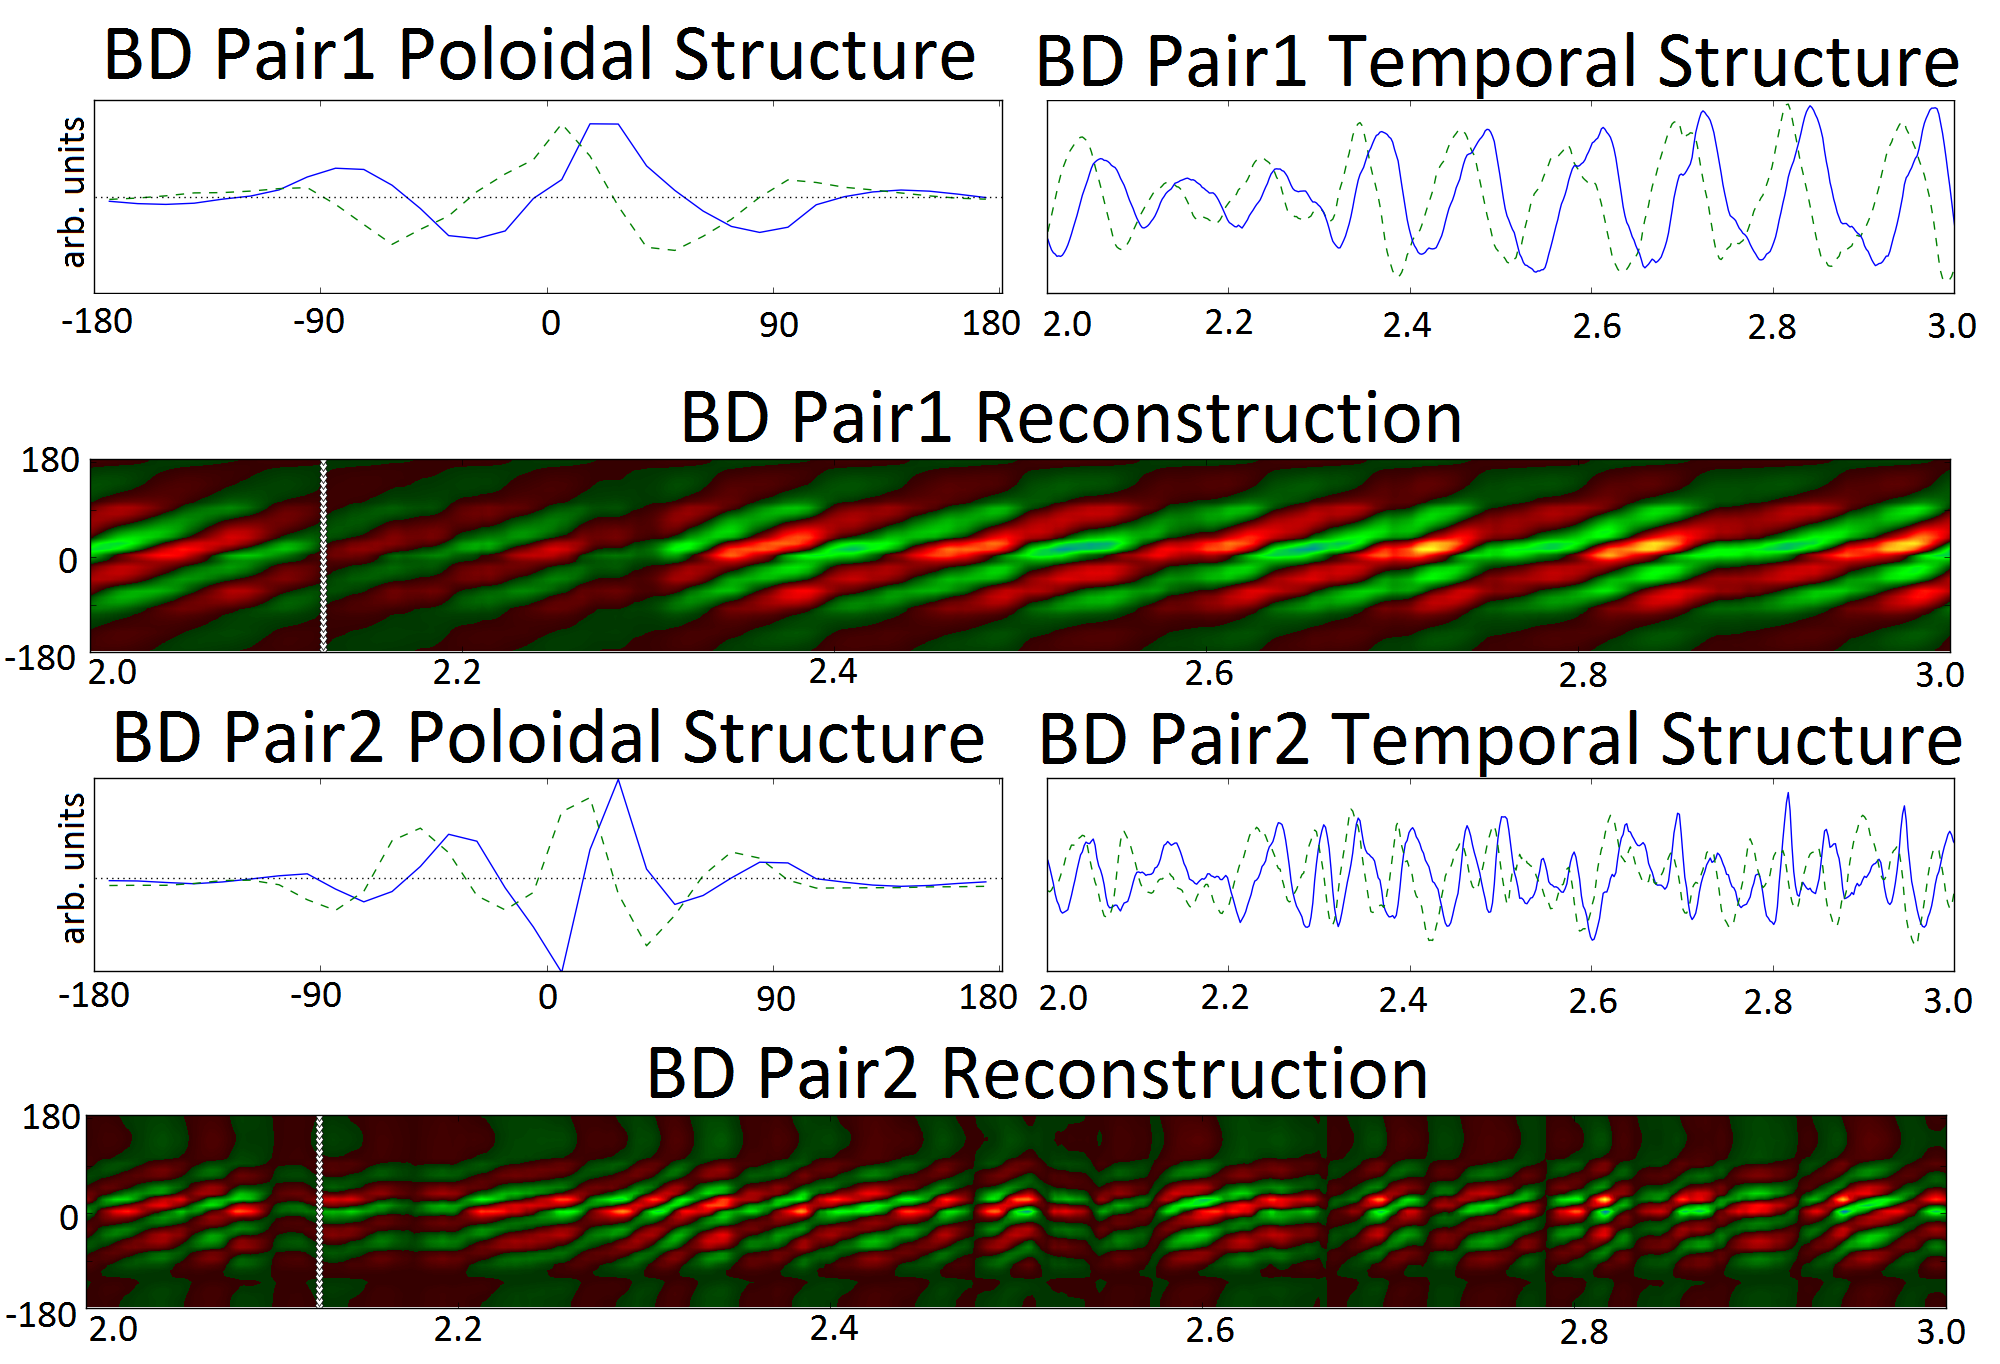
\includegraphics[width=1\columnwidth]{85402_bd_reconstructions.png}\\

\end{center}
\item This method is robust to dead sensors, sensor gain/alignment errors, and the modes' finite m spectrum due to toroidicity
\subitem - These effects are included in the mode and do not give rise to artifacts, as would occur with Fourier transforms
\item Mode is isolated from as-measured fluctuations
\subitem - If mode-sensor coupling is low, mode amplitude at that sensor will be attenuated
\subitem - Shaped plasmas are created outboard; sensors near $180^{\circ}$ less well-coupled than those near $0^{\circ}$\\


\section{Modeling}
\subsection{Equilibria Reconstruction}
\item Equilibrium/mode reconstructions using TokaMac and DCON predict significant changes to mode structure on the surface of a shaped plasma, especially near the X-point
\begin{center}

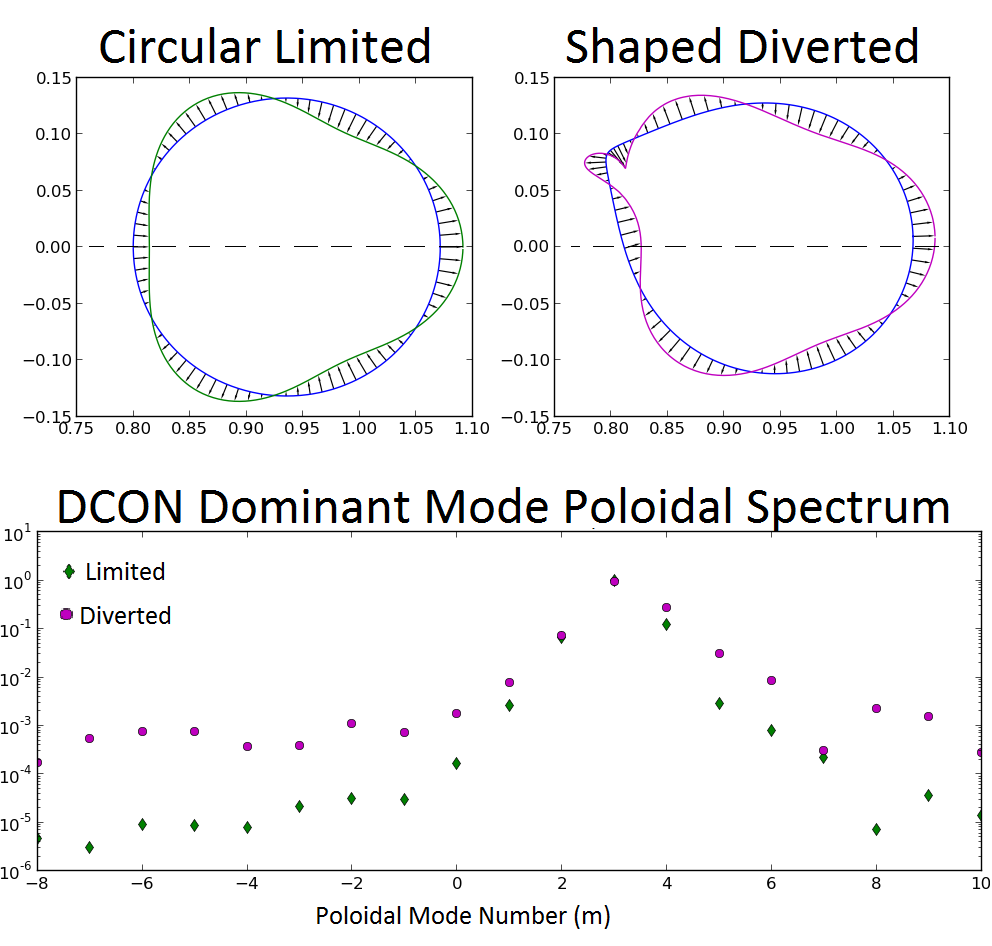
\includegraphics[width=1\columnwidth]{Dcon_surfaces_n1_dom_85385_85402}\\

\end{center}

\subsection{Forward Modeling of Fluctuations}
\item HBT-EP Poloidal sensor arrays are conformal to \textbf{circular} plasmas, centered in the vacuum vessel
\subitem - Sensor coupling to outboard, shaped plasmas will vary poloidally and will be weak near X-point
\subitem - Stabilizing shells will reduce $B_r$ signal for shell-mounted sensors ($-90 \geq \theta	\leq 90$), will enhance $B_p$ signal
%\item Poloidal variation of plasma-sensor coupling requires forward modeling to compare mode on the plasma to mode as-measured
\item VALEN is necessary to model sensor pickup of mode using a full 3-D representation of HBT-EP's conducting structures
\subitem - Includes effects of poloidally variable sensor/mode coupling, mode rotation, and eddy currents due to shells, vacuum vessel, etc.

\begin{center}

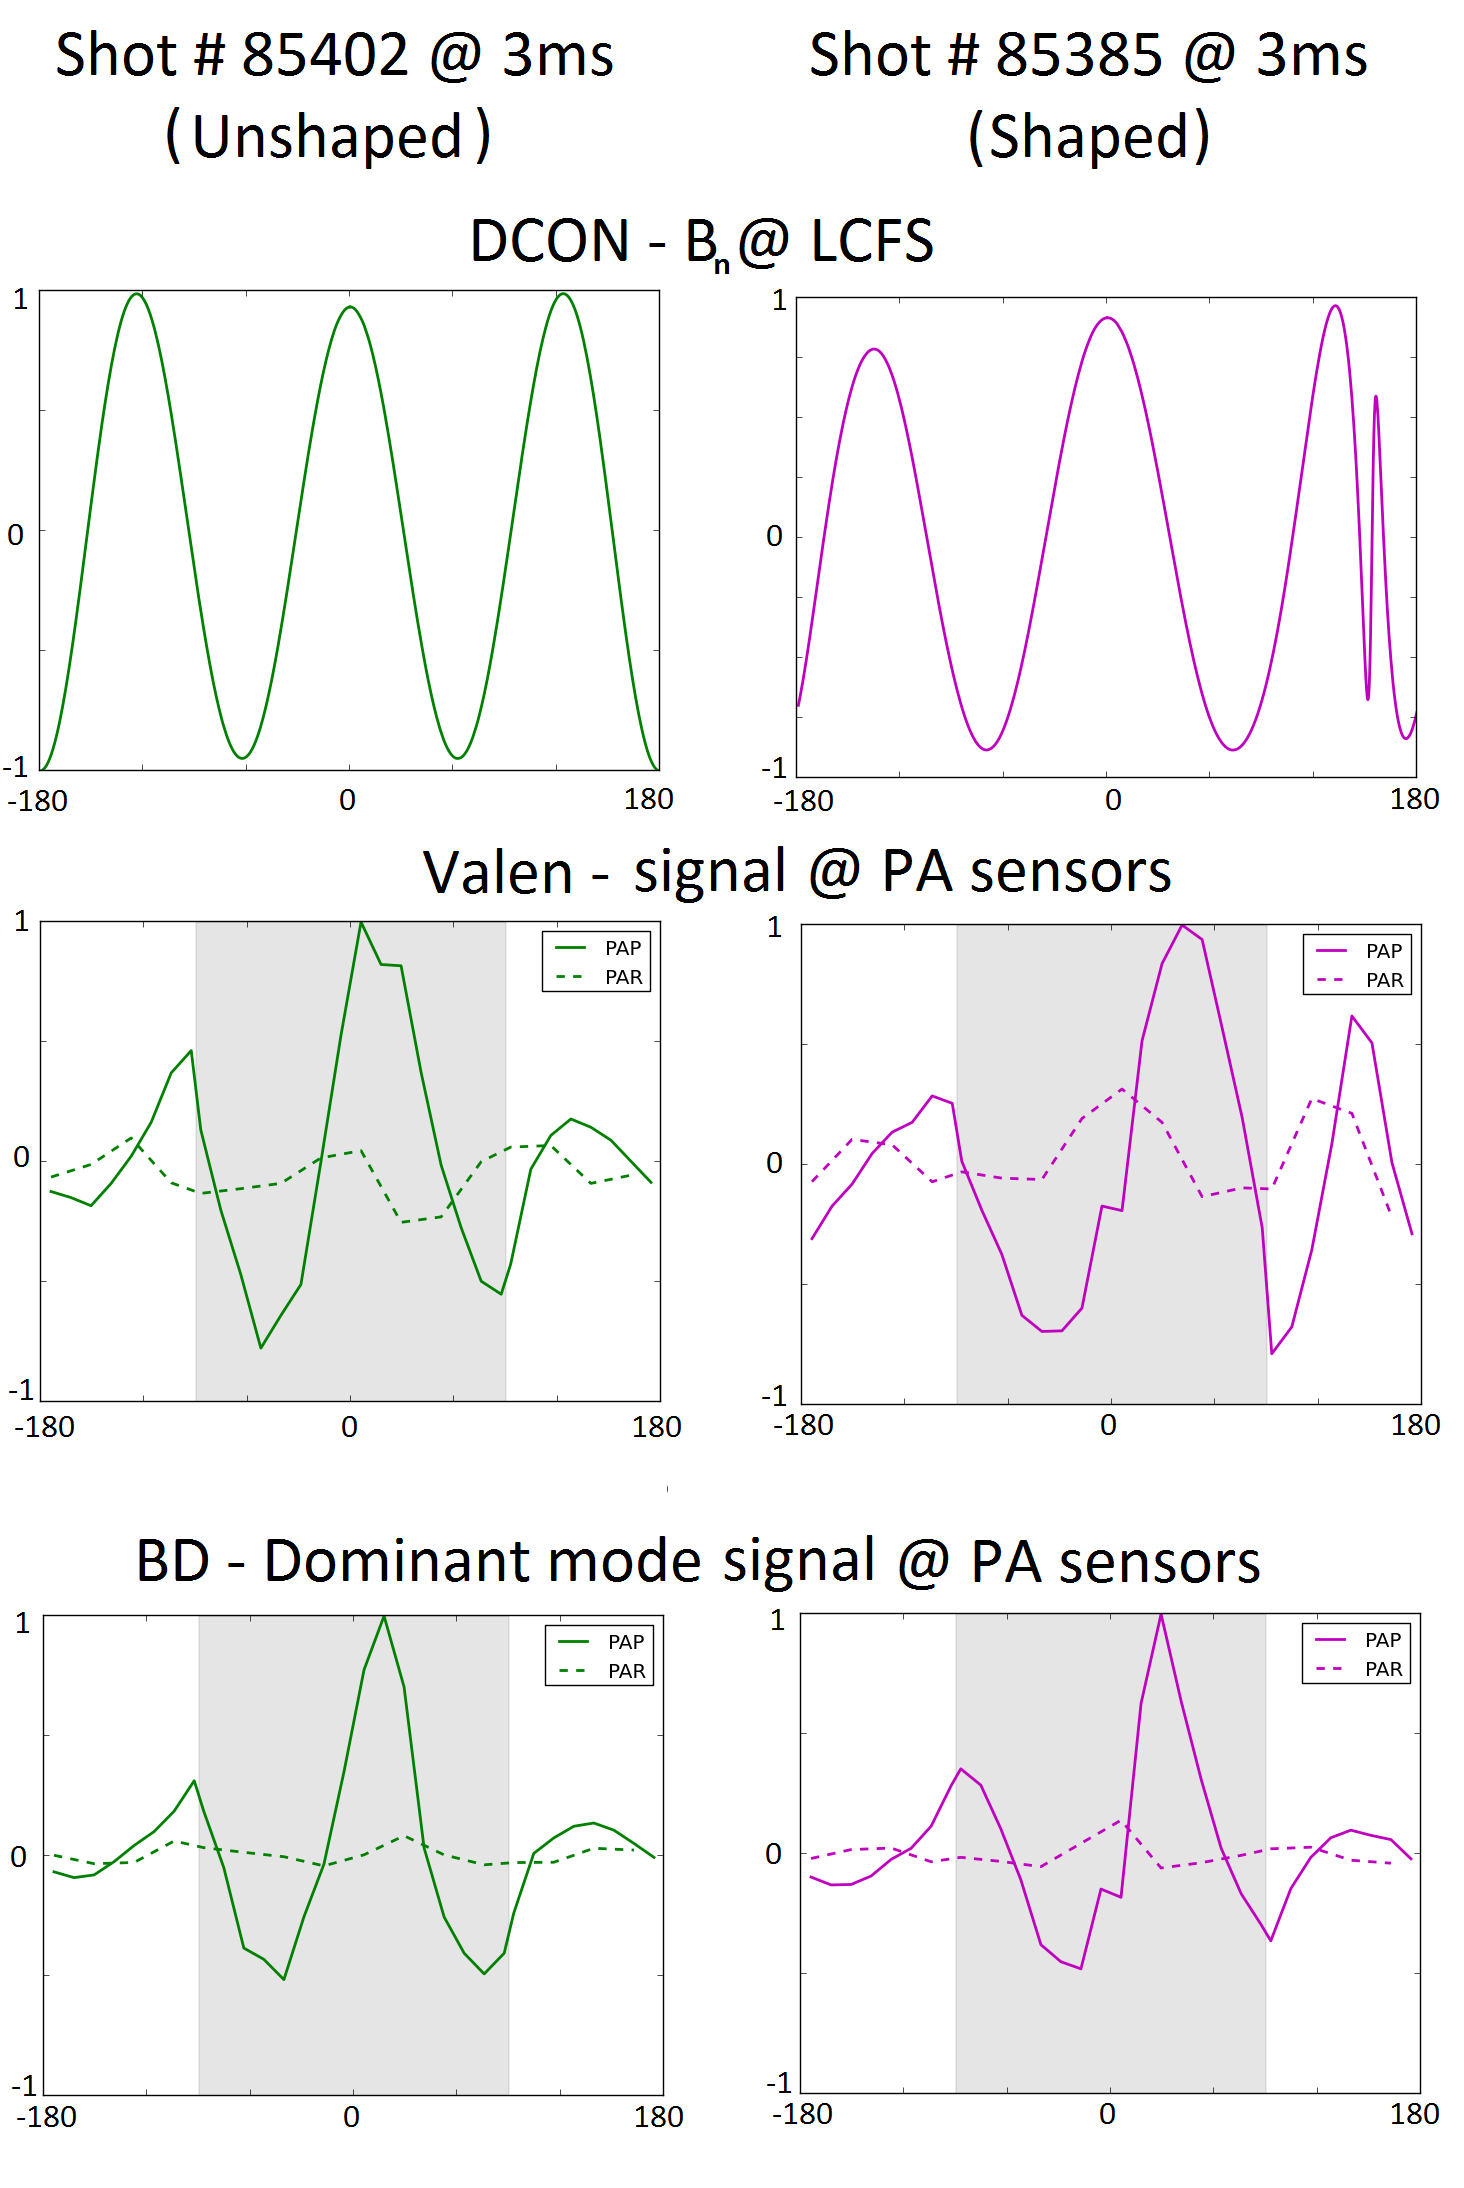
\includegraphics[width=1\columnwidth]{Modeling_to_reality_comparison.png}\\

\end{center}
\item Predicitons of VALEN based on DCON output are compared to actual modes measured in the plasma
\subitem - Shell amplification of $B_p$, reduction of $B_r$ is predicted and observed
\subitem - Measured $B_r$ amplitude is smaller than predicted by VALEN
\subitem - Difficulty in measuring $4^{th}$ peak is likely.  May be possible to change equilibrium parameters (MR, IP) to increase sensor coupling near X-point

\item Poloidal mode spectrum is seen to broaden as expected for $ m>3$, but low-m broadening is not observed
\begin{center}
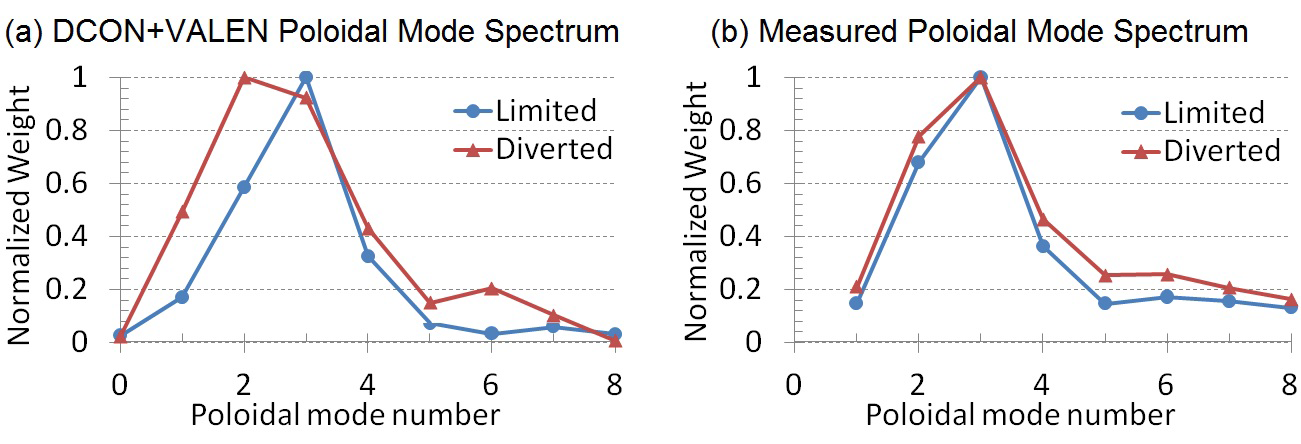
\includegraphics[width=1\columnwidth]{fig2_mode_spectrum_REV2.png}
\end{center}

\section{Resonant Magnetic Perturbation}
\item RMPs applied with HBT-EP's control coil array can excite one or more natural modes, allowing further investigation into mode structure and multimode dynamics\\
\item Up to 20G of $B_r$ is available, and imposing RMP as a phase-flip allows contrast of phases - equivalent to 40G\\
\item RMPs on HBT-EP have been imposed as:
\begin{equation}
A\;f(t)\;cos(m\theta_i+n\phi_i)
\end{equation}
\item VALEN calculations show that coupling varies poloidally, due to both shaping and rotation-induced eddy currents - RMP amplitude should be $A(\theta_i)$
\begin{center}
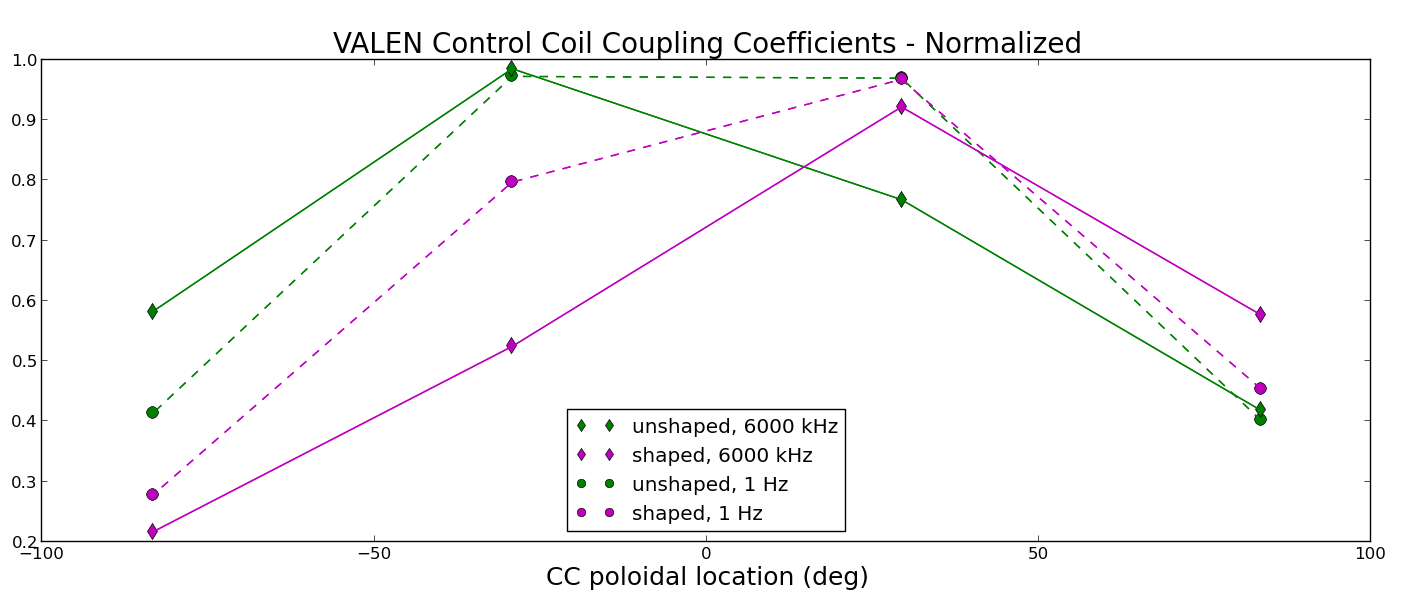
\includegraphics[width=1\columnwidth]{VALEN_CC_coupling}
\end{center}

\section{Conclusions \& Future Work}
\item HBT-EP has been upgraded with a divertor coil which has successfully been used to create a variety of shaped plasmas
\item For the first time, HBT-EP has used TokaMac, DCON, and VALEN together to model an equilibrium and its MHD modes, and from that the expected sensor signal, for comparison to direct measurements
\item Differences in measured mode structure between shaped and unshaped plasmas are subtle, but this is in agreement with predictions
\item We will continue to develop shaped equilibria for improved lifetime, positional stability, and sensor resolution near X-point
\item We will apply RMPs to enhance sensor/mode coupling, and detect differences in shaped plasma's resonant mode spectrum w.r.t. circular
\item VALEN predictions for control coil coupling will be used when choosing RMP structure to improve control efficiency
\begin{thebibliography}{9}%
\large
\bibitem{Maurer}D.\thinspace A.~Maurer, {\it et.\thinspace al.\/}, Plas. Phys.~Control. Fusion,
(2011) Vol. 53 Iss. 7
\bibitem{Levesque} J. P. Levesque, \emph{Multimode Structure of Resistive Wall Modes Near the Ideal Wall Stability Limit}, Ph.D. Thesis, Columbia University (2012).
\bibitem{Shiraki} D. Shiraki, \emph{High Resolution MHD Spectroscopy of External Kinks in a Tokamak Plasma}, Ph.D. Thesis, Columbia University (2012)
\end{thebibliography}
                                                                   
       
{\flushleft\LARGE\color{lnavy}\sf\bfseries{Acknowledgements}}

Design, fabrication, and installation were all aided greatly by the contributions of Nick Rivera and James Andrello\\
\newline
This work was supported by DOE grant DE-FGO2-86ER53222
\end{itemize}
\end{multicols}
\end{document}